\documentclass[12pt, a4paper]{article}

\usepackage[hmargin=2.5cm, vmargin=2cm]{geometry}
\usepackage{amsthm, amssymb, mathtools, yhmath, graphicx}
\usepackage{fontspec, type1cm, titlesec, titling, fancyhdr, tabularx}
\usepackage{color}
\usepackage{unicode-math}
\usepackage{float}
\usepackage{subfig}
\usepackage{hhline}
\usepackage{comment}
\usepackage[abbreviation,per-mode=symbol]{siunitx}
\usepackage{csvsimple}
\usepackage{subcaption}

\usepackage[CheckSingle, CJKmath]{xeCJK}
\usepackage{CJKulem}
\usepackage{enumitem}
\usepackage{tikz}
\usepackage[siunitx]{circuitikz}
\usepackage{wrapfig}
%\setCJKmainfont[BoldFont=cwTex Q Hei]{cwTex Q Ming}
%\setCJKsansfont[BoldFont=cwTex Q Hei]{cwTex Q Ming}
%\setCJKmonofont[BoldFont=cwTex Q Hei]{cwTex Q Ming}
\setCJKmainfont[BoldFont=cwTeX Q Hei]{cwTeX Q Ming}

\def\normalsize{\fontsize{12}{18}\selectfont}
\def\large{\fontsize{14}{21}\selectfont}
\def\Large{\fontsize{16}{24}\selectfont}
\def\LARGE{\fontsize{18}{27}\selectfont}
\def\huge{\fontsize{20}{30}\selectfont}

%\titleformat{\section}{\bf\Large}{\arabic{section}}{24pt}{}
%\titleformat{\subsection}{\large}{\arabic{subsection}.}{12pt}{}
%\titlespacing*{\subsection}{0pt}{0pt}{1.5ex}

\parindent=24pt

\DeclarePairedDelimiter{\abs}{\lvert}{\rvert}
\DeclarePairedDelimiter{\norm}{\lVert}{\rVert}
\DeclarePairedDelimiter{\inpd}{\langle}{\rangle}
\DeclarePairedDelimiter{\ceil}{\lceil}{\rceil}
\DeclarePairedDelimiter{\floor}{\lfloor}{\rfloor}

\newcommand{\unit}[1]{\:(\text{#1})}
\newcommand{\df}[1]{\mathop{}\!\mathrm{d^#1}}
\newcommand{\img}{\mathrm{i}}
\newcommand{\dD}{\mathrm{d}}
\newcommand{\dI}{\,\mathrm{d}}
\newcommand{\paral}{\mathbin{\|}}

\title{ \bf {\Huge 電子電路實驗3: VTC of CMOS Amplifier Circuits  }\\ 實驗結報}
\author{B02901178 江誠敏}

\begin{document}

\maketitle


\section{實驗結果}

\subsection{Bode plot}
\begin{figure}[H]
\begin{center}
  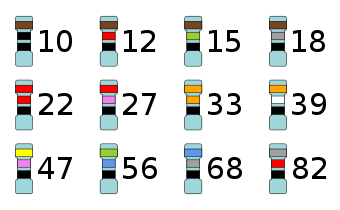
\includegraphics[width=.8\textwidth]{fig1.pdf}
\end{center}
\caption{Bode plot}
\label{fig:}
\end{figure}


\section{結報問題}

\begin{enumerate}[itemsep=20pt, topsep=10pt]

  \item {如何透過量測方式判別 BJT 與 MOS 的腳位(請詳述之)。Ex: BJT 可用指針電表量測。} \\[10pt]
    答:
    \begin{enumerate}[(a)]
      \item BJT. 
        \begin{itemize}
          \item 首先判斷哪一個腳位是 B ,假設未知腳位是 $1, 2, 3$ , 以電阻檔位量測所有 $(i, j)$ 是否導通。
            如果發現一對正接反接都無法導通(如 $(1, 2), (2, 1)$ ),那剩下的一隻腳位(即 $3$) 就是 B 。
          \item 利用以知的 B 腳位,和剩下的任一隻腳位 $j$ 以電阻檔測量哪一個方向可以導通,
            進而判斷是 pnp 還是 npn。
          \item 最後假設剩下的兩個腳位是 $i, j$ , 將 $i, \text{B}$ 接在一起,之後 $i, \text{B}$ 端和 $j$ 端以
            電阻檔測量兩個方向是否有一邊可導通,如果可以,則 $i$ 是 E 端,如果皆不能導通,則 $i$ 是 C 端。
            如此便可確定所有檔位。
        \end{itemize}
      \item MOS. 
        \begin{itemize}
          \item 首先判斷哪一個腳位是 G ,假設未知腳位是 $1, 2, 3$ , 以電阻檔位量測所有 $(i, j)$ 是否導通。
            如果發現一對可導通(如 $(1, 2), (2, 1)$ ),那剩下的一隻腳位(即 $3$) 就是 G 。
          \item 最後假設剩下的兩個腳位是 $i, j$ , 將 $i, \text{B}$ 接在一起,之後 $i, \text{B}$ 端和 $j$ 端以
            電阻檔測量電阻 $R_1$,接著 $i, j$ 互換同樣方式測量得電阻 $R_2$
            ,如果 $R_1 > R_2$ ,則 $i$ 是 D 端,否則 $i$ 是 S 端。
            如此便可確定所有檔位。
        \end{itemize}
    \end{enumerate}

  \item {請列舉5項常見的IC封裝方式,並說明其優缺點。} \\[10pt]
    答:
    \begin{enumerate}
      \item 雙列直插封裝:封裝成的外形為長方形,並在兩側則有兩排平行的金屬引脚。優點是可以插在面包
        板上,適合極簡單的開發使用。
      \item 插針網格陣列:將集成電路包裝在底面是排列成正方形的插針的瓷片內,最後這些插針可以插入或焊接到電路板上對應的插座中,適合於需要頻繁插拔的應用場合。
      \item 球柵陣列封裝:由插針網格陣列改良而來,本來在封裝底部的引腳由錫球所取代。優點有可以有高密度的引腳、高導熱避免IC過熱和
        低電感引腳。
      \item 平面網格陣列封裝:特點是其針腳位於插座上而非積體電路上,可避免針腳損壞。
      \item 多晶片模組:此種封裝能在一次容納兩個或兩個以上的晶片。這也是他的優點。
    \end{enumerate}

  \item {何謂 3D IC ? 請說明在目前主流技術中 TSV 的優缺點與未來的發展。} \\[10pt]
    答:\\
    現在的 IC 主要都是平面型的設計,但電晶體元件的大小已經難以在繼續縮小下去。因此
    如果希望單位體積的電晶體數量可以增加,可能必須考慮 3D 的設計方式了。

    TSV 是在晶片鑽出小洞,從底部填充入金屬,接著在矽晶圓上以蝕刻或雷射方式鑽孔,最後以導電材料填滿。
    優點是可以更低的成本提高系統的整合與效能,缺點是TSV孔徑較大,使得TSV密度無法提高。未來可能會
    朝向提高蝕刻速度、較好的蝕刻輪廓、降低成本、提升產能等等發展。
    
  \item {請繪出CMOS的物理元件結構圖,並說明閉鎖效應的成因、機制。} \\[10pt]
    答:\\
    \begin{figure}[H]
    \begin{center}
      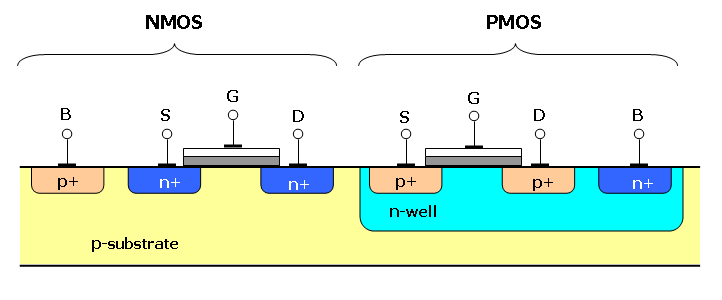
\includegraphics[width=0.7\textwidth]{cmos.png}
    \end{center}
    \caption{}
    \end{figure}

    \begin{figure}[H]
    \begin{center}
      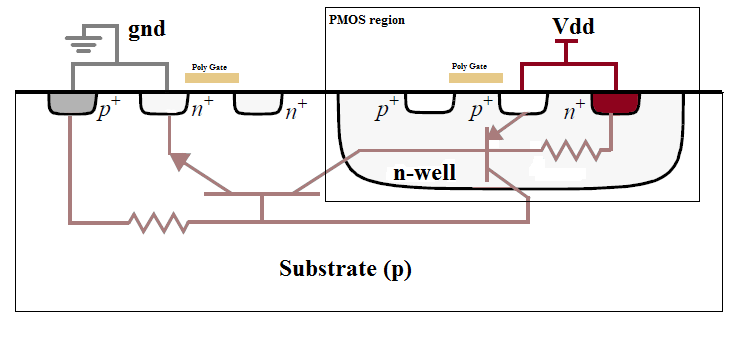
\includegraphics[width=0.7\textwidth]{latchup.png}
    \end{center}
    \caption{}
    \end{figure}

    成因是因為通常 CMOS 的 NMOS, PMOS 部分都是弄在同一塊板子上,所以其實會互相影響,嚴重甚至
    會造成整個電路失效。

  \item {What kind of capacitance are $C_\pi$ and $C_\mu$ shown in Fig. 1? How are they generated? Which one of them is larger ?
      Should they be opened or shorted as operated in low frequency? Which part of frequency band (low or high) 
do they determine? } \\[10pt]
    答:\\
    $C_\mu$ is the capacitor between C and B due to {\bf junction capacitance}. \\
    $C_\pi$ is the capacitor between E and B due to {\bf junction capacitance} and {\bf diffusion capacitance}. \\
    Typically $C_\pi$ is larger.  \\
    They should be open in low frequency. \\
    They determine the high frequency band.

  \item{What kind of capacitance are $C_1$ , $C_2$ , and $C_3$ shown in Fig. 2? What are they used for? Should they be opened or shorted as operated in high frequency? Which part of frequency band (low or high) do they determine? } \\[10pt]
    答:\\
    What kind... 啊不就實驗用的一般電容…
    They are used to block the DC offset signal. \\
    They should be closed in high frequency. \\
    They determine the low frequency band. \\

  \item{What kind of amplifier (configuration CE, CB, CC) is appropriate for operating in low/high/Impedance transformation frequency? Why?}
    \\[10pt]
    CE is appropriate to operating in low frequency, because it has the greatest voltage gain. \\
    CB is appropriate to operating in high frequency, because it has the highest cutoff frequency. \\
    CC is appropriate to operating in inpedance transformation, because its output resistance is very small.

\end{enumerate}

\section{心得}
這次的實驗其實很吃運氣。一開始我們這排大部分的人都做的很順利,除了一個人之外。他不知道為什麼怎麼做,
波形看起來就是非常奇怪。電路檢查了半天,就是什麼bug都沒有發現。後來我就跟他說「你甘脆把所有元件都換一
輪看看。」沒想道他才換了一個 BJT ,瞬間一切都 work 了! 他當場倒地不起,痛哭流涕。 那時候我們其他人
幾乎都做完了。 這個故事告訴我們,在一般的事情上,發現問題時,最好先檢查自已有沒有問題,不要一開始就覺
得是別人的錯,唯有做電電實驗時必須反過來!
\end{document}

